\documentclass{beamer}

\usetheme{Boadilla}

\usepackage{hyperref}
\hypersetup{colorlinks=true}

\begin{document}

\title{Introduction to ROS} 
\author{Kurbakov Dmytro, Slonina Michal}

\date{11.10.2019}

\begin{frame}
\titlepage
\end{frame}

\begin{frame}
All slides are available here:\\
\url{https://github.com/project-omicron/robocar/}
\end{frame}

\section{History of ROS} 
\begin{frame}
\begin{center}
\Huge History of ROS
\end{center}
\end{frame}
\begin{frame}{ROS motivation}
\begin{tabular}{ll}
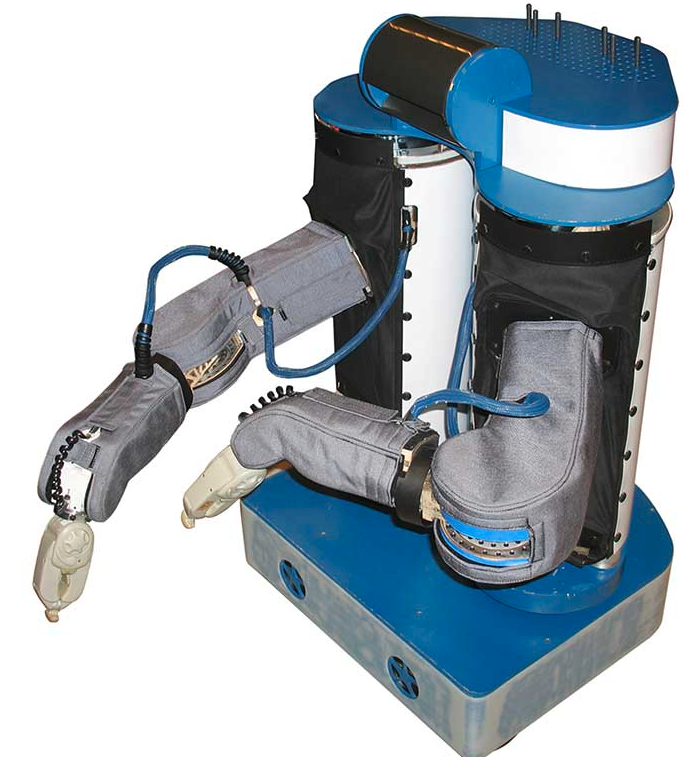
\includegraphics[scale=0.08]{images/pr1_clean} 
&
\begin{tabular}{l}
No single solution how to program robots \\
\\
Eric Berger and Keenan Wyrobek, PhD students at \\
Stanford, build PR1 (Personal Robot One) and began\\
to work on software from it, borrowing the best \\
practices from other early open source robotic \\
software frameworks \\
\\
Early funding of US\$50,000 was provided by Joanna \\
Hoffman and Alain Rossmann,  which supported the \\
development of the PR1
\end{tabular}
\end{tabular}
\end{frame}

\begin{frame}{Outcome}
\begin{tabular}{ll}
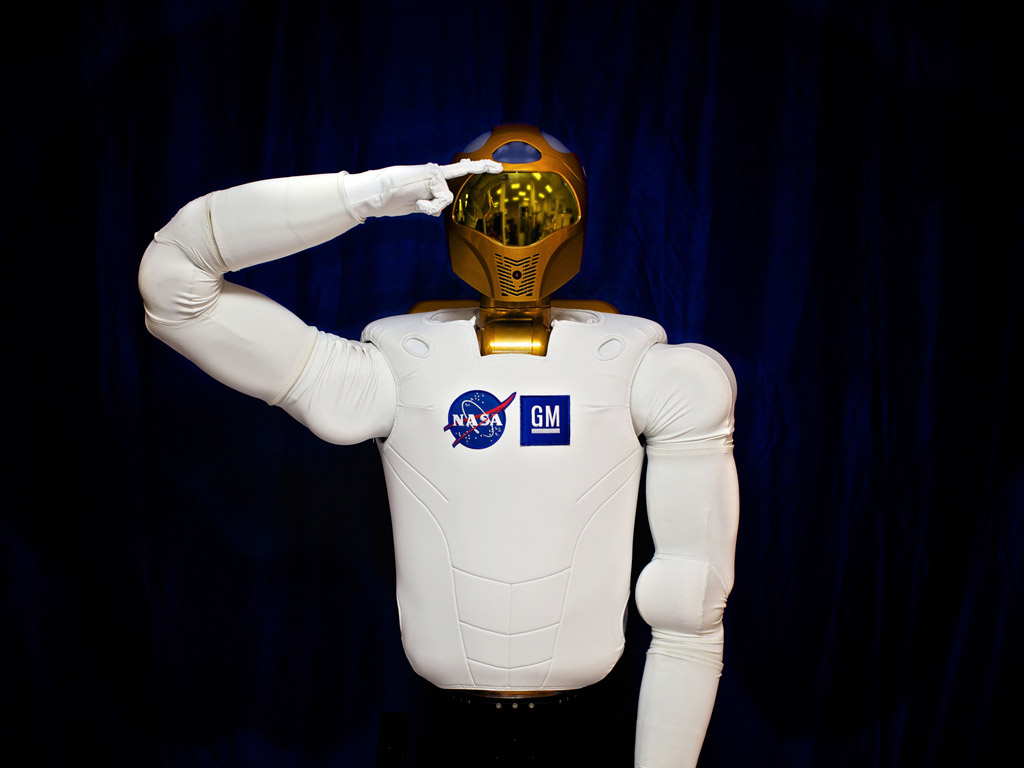
\includegraphics[scale=0.08]{images/robonaut} 
&
\begin{tabular}{l}
ROS provides rich selection of packages\\
\\
ROS has a huge set of tools to design robots\\
\\
A new version of ROS every year\\
\\
ROSCons occurres every year since 2012\\
\\
Robotnaut 2: first ROS based robot in space\\
\\
ROS2 was released\\
\end{tabular}
\end{tabular}
\end{frame}


\section{Structure of ROS}
\begin{frame}
\begin{center}
\Huge Structure of ROS
\end{center}
\end{frame}

\subsection{Catkin workspace}
\begin{frame}{What is a workspace in ROS}
\textbf{Workspace} is the folder inside which you are going to be actively developing. Keeping things in a folder with connected development helps keep separation of development models
\vfill
\textbf{Catkin} is a low-level build system macros and infrastructure for ROS
\vfill
\textbf{Catkin workspace} is a folder where you modify, build, and install catkin packages
\vfill
For more information, check: \href{http://wiki.ros.org/catkin}{ROS catkin documantation}
\end{frame}

\begin{frame}{Introduction to catkin\_init\_workspace and catkin\_make}
\textbf{catkin\_init\_workspace} initializes a catkin workspace by creating a top level CMakeLists.txt
\vfill
\textbf{catkin\_make} is a convenience tool for building code in a catkin workspace. catkin\_make follows the standard layout of a catkin workspace
\end{frame}

\subsection{Node}
\begin{frame}{Robot architecture in ROS, example}
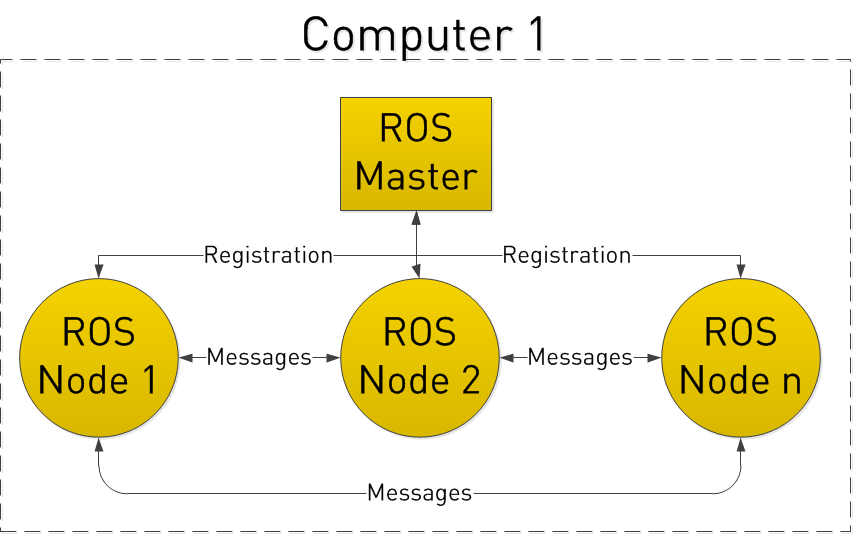
\includegraphics[scale=0.35]{images/ros}
\end{frame}

\begin{frame}{ROS Master}
The ROS Master provides naming and registration services to the rest of the nodes in the ROS system.

\begin{itemize}
\item Tracks publishers and subscribers nodes
\item Tracks topics
\item Tracks services
\item Provide parameter server\\
Shared, multi-variate dictionary, accessible via network APIs.\\
Nodes use this server to store and retrieve parameters at runtime.\\
\end{itemize}
\end{frame}

\begin{frame}{Publisher vs. Subscriber}
\textbf{Publisher}: Node that puts information to the topic
\vfill
\textbf{Subscriber}: Node that checkes if the information arrives to the topic. Once the information arrived, it can react correspondingly
\vfill
In ROS, every note can be a publisher, subscriber or both
\vfill
For more info, check \href{http://wiki.ros.org/ROS/Tutorials/WritingPublisherSubscriber\%28python\%29}{here}
\end{frame}

\subsection{Topic}
\begin{frame}{What is the topic in ROS}
\textbf{Topic} is a named buse over which nodes exchange messages
\vfill
Each topic is strongly typed by the ROS message type
\vfill
ROS currently supports TCP/IP-based and UDP-based message transport
\begin{enumerate}
\item TCPROS is the default transport used in ROS 
\item UDP-based transportis currently only supported in roscpp
\end{enumerate}
\end{frame}

\begin{frame}{Introduction to the command rostopic}
\textbf{rostopic} is a command-line tool for interacting with ROS topics
\vfill
Once you run the robot, you can see all available topics\\
\textit{rostopic list}
\vfill
Current value in the topic\\
\textit{rostopic echo /topic\_name}
\vfill
Information about the frequenze of the topic\\
\textit{rostopic hz /topic\_name}
\vfill
More information: \href{http://wiki.ros.org/rostopic}{ROS Topic}
\end{frame}

\subsection{Service}
\begin{frame}{What is the service in ROS}
Request/reply is done via a Service, which is defined by a pair of messages: one for the request and one for the reply.
\vfill
Services are defined using srv files.
\vfill
Generally saying: service is the RPC in ROS.
\end{frame}

\begin{frame}{Introduction to the command rosservice}
\textbf{rosservice} contains the rosservice command-line tool for listing and querying ROS Services
\vfill
List all the services that are currently available\\
\textit{rosservice list}
\vfill
Print information about specified service
\textit{rosservice info /rosout}
\vfill
Call a service from the command line\\
\textit{rosservice call /service\_name service-args}
\vfill
For more information: \href{http://wiki.ros.org/rosservice}{ROS Service}
\end{frame}

\begin{frame}{MUX}
\textit{mux} is a ROS node that subscribes to a set of incoming topics and republishes incoming data from one of them to another topic
\vfill
Example:\\
We use mux to switch from AI controller to human controller.
\vfill
More information and examples: \href{http://wiki.ros.org/topic_tools/mux}{ROS mux}
\end{frame}

\subsection{How to run the robot}
\begin{frame}{roscore and rosrun}
\textbf{roscore} is a collection of nodes and programs that are pre-requisites of a ROS-based system. You \textbf{must} have a roscore running in order for ROS nodes to communicate.

\vfill

\textbf{rosrun} allows you to run an executable in an arbitrary package from anywhere without having to give its full path or cd/roscd there first.
\vfill
Example:\\
\textit{roscore}\\
\textit{rosrun package node \_parameter:=value}
\vfill
For more information, see \href{https://wiki.ros.org/rosbash\#rosrun}{ROS rosrun}, \href{https://wiki.ros.org/roscore}{ROS roscore}
\end{frame}

\begin{frame}{roslaunch}
\textbf{roslaunch} is a tool for easily launching multiple ROS nodes locally and remotely via SSH, as well as setting parameters on the Parameter Server.
\vfill
roslaunch takes in one or more XML configuration files (with the .launch extension) that specify the parameters to set and nodes to launch, as well as the machines that they should be run on.
\vfill
Example:\\
\textit{roslaunch package\_name file.launch}
\vfill
For more information, see \href{https://wiki.ros.org/roslaunch}{ROS roslaunch}
\end{frame}

\section{Introduction to Omicron}
\begin{frame}
\begin{center}
\Huge Project OMICRON
\end{center}
\end{frame}

\subsection{High level architecture}
\begin{frame}{High level description of nodes}
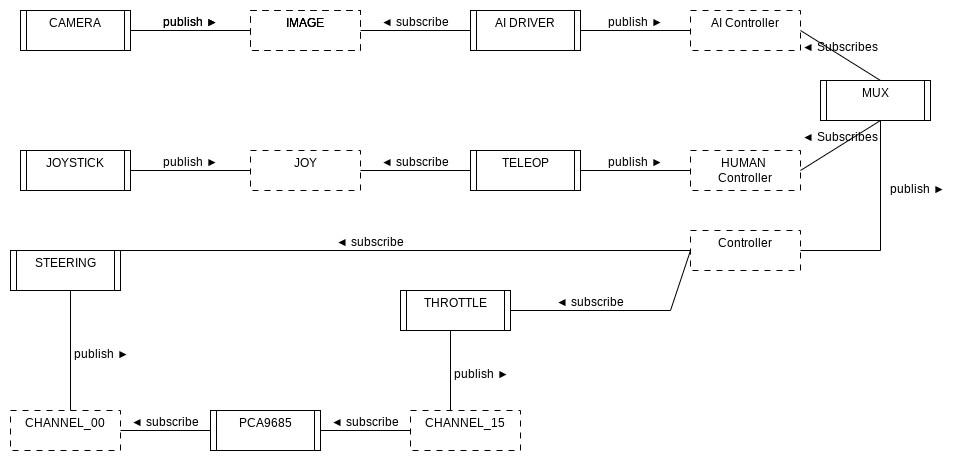
\includegraphics[scale=0.35]{images/omicron_graph} 
\end{frame}

\begin{frame}{Thank you!}
\textbf{Contacts}\\
\vfill
Kurbakov Dmytro\\
Email: dmytro.kurbakov@tomtom.com\\
LinkedIn: \url{https://linkedin.com/in/dmytro-kurbakov/}\\
\vfill
Slonina Michal\\
Email: michal.slonina@tomtom.com\\
LinkedIn: \url{https://www.linkedin.com/in/michalslonina/}\\
\end{frame}


\begin{frame}{Whant to know more? Useful links}
\href{https://spectrum.ieee.org/automaton/robotics/robotics-software/the-origin-story-of-ros-the-linux-of-robotics}{The Origin Story of ROS, the Linux of Robotics}\\
\href{https://www.ros.org/history/}{ROS History, ROS.org}\\
\href{https://en.wikipedia.org/wiki/Robot_Operating_System}{ROS, wiki page}\\
\href{http://wiki.ros.org/Industrial/Tutorials}{ROS Industrial}
\href{https://wiki.ros.org/ROS/Tutorials/WritingPublisherSubscriber\%28python\%29}{ROS Tutorial for publisher and subscriber}
\end{frame}


\end{document}

